\documentclass[11pt, a4paper]{article}

% --- Core Packages ---
\usepackage[utf8]{inputenc}
\usepackage{amsmath, amssymb, amsfonts}
\usepackage{geometry}
\geometry{margin=0.75in}
\usepackage{xcolor}
\usepackage{tikz}
\usetikzlibrary{3d, calc, patterns, arrows.meta, shapes.geometric}

% --- Font Support for Bengali (Compile with XeLaTeX or LuaLaTeX) ---
\usepackage{fontspec}
\setmainfont{Kalpurush}[
    Script=Bengali,
    Path = ./ , % Adjust font path as necessary for your system
    FallbackFont = {FreeSerif}
]

\begin{document}

% ==================== QUESTION 1 ====================
\subsection*{প্রশ্ন ১ / Question 1}
\textbf{প্রশ্ন:} যদি একটি গতিশীল কণার অবস্থান ভেক্টর $\vec{r} = bt^2\hat{i} + ct^3\hat{j}$ হয়, যেখানে $b$ ও $c$ দুটি ধনাত্মক ধ্রুবক এবং $t$ হলো সময়। কখন কণাটির বেগ ভেক্টরটি x ও y অক্ষের ধনাত্মক দিকের সাথে সমান কোণে অর্থাৎ $45^\circ$ কোণে অবস্থান করবে? [If the position vector of a moving particle is $\vec{r} = bt^2\hat{i} + ct^3\hat{j}$, where $b$ and $c$ are positive constants and $t$ is time, at what time will the velocity vector of the particle make an equal angle of $45^\circ$ with the positive x and y axes?] [৬]

\vspace{0.8em}
\textbf{সমাধান / Solution:}

অবস্থান ভেক্টর $\vec{r}$ কে সময়ের সাপেক্ষে অন্তরীকরণ (differentiation) করলে বেগ ভেক্টর পাওয়া যায়:

$$\vec{v} = \frac{d\vec{r}}{dt} = \frac{d}{dt}(bt^2\hat{i} + ct^3\hat{j})$$

$$\vec{v} = 2bt\hat{i} + 3ct^2\hat{j}$$

এখানে বেগের x-অংশ $v_x = 2bt$ এবং y-অংশ $v_y = 3ct^2$।

শর্তানুসারে, বেগ ভেক্টরটি x ও y অক্ষের সাথে $45^\circ$ কোণে থাকবে। অতএব:

$$\tan 45^\circ = \frac{v_y}{v_x}$$

$$\Rightarrow 1 = \frac{3ct^2}{2bt}$$

যেহেতু $t > 0$ (সময় ধনাত্মক), উভয় পক্ষকে $t$ দ্বারা ভাগ করে পাই:

$$\Rightarrow 3ct = 2b$$

$$\Rightarrow t = \frac{2b}{3c}$$

\textbf{উত্তর:} $t = \frac{2b}{3c}$ সময়ে বেগ ভেক্টরটি x ও y অক্ষের সাথে $45^\circ$ কোণে অবস্থান করবে।

\vspace{1em}
\begin{center}
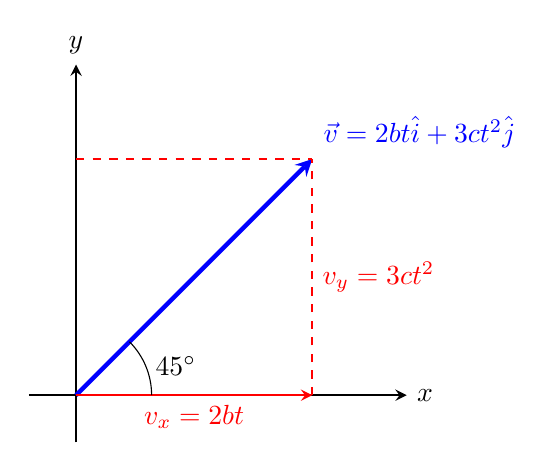
\begin{tikzpicture}[scale=1.2, >=stealth]
    \draw[->, thick] (-0.5,0) -- (3.5,0) node[right] {$x$};
    \draw[->, thick] (0,-0.5) -- (0,3.5) node[above] {$y$};
    \draw[->, ultra thick, blue] (0,0) -- (2.5,2.5) node[above right] {$\vec{v} = 2bt\hat{i} + 3ct^2\hat{j}$};
    \draw[dashed, red, thick] (2.5,0) -- (2.5,2.5) node[midway, right] {$v_y = 3ct^2$};
    \draw[dashed, red, thick] (0,2.5) -- (2.5,2.5);
    \draw[->, red, thick] (0,0) -- (2.5,0) node[midway, below] {$v_x = 2bt$};
    \draw (0.8,0) arc (0:45:0.8) node[midway, right] {$45^\circ$};
\end{tikzpicture}
\end{center}

\vspace{1em}
\noindent\rule{\textwidth}{0.4pt}
\vspace{1em}

% ==================== QUESTION 2 ====================
\subsection*{প্রশ্ন ২ / Question 2}
\textbf{প্রশ্ন:} ত্রিমাত্রিক কার্তেসীয় স্থানাঙ্ক ব্যবস্থায় তিনটি বিন্দু A, B ও C এর অবস্থান ভেক্টর যথাক্রমে $\vec{OA} = \hat{i} + 2\hat{j} - 3\hat{k}$, $\vec{OB} = 3\hat{i} - 4\hat{j} + 5\hat{k}$ এবং $\vec{OC} = 5\hat{i} - 10\hat{j} + 13\hat{k}$। ভেক্টর বীজগণিত ব্যবহার করে প্রমাণ করো যে, বিন্দু তিনটি সমরেখিক (collinear)। [In a three-dimensional Cartesian coordinate system, the position vectors of three points A, B, and C are $\vec{OA} = \hat{i} + 2\hat{j} - 3\hat{k}$, $\vec{OB} = 3\hat{i} - 4\hat{j} + 5\hat{k}$, and $\vec{OC} = 5\hat{i} - 10\hat{j} + 13\hat{k}$, respectively. Using vector algebra, prove that the three points are collinear.] [৬]

\vspace{0.8em}
\textbf{সমাধান / Solution:}

প্রথমে $\vec{AB}$ এবং $\vec{BC}$ ভেক্টর দুটি নির্ণয় করি:

$$\vec{AB} = \vec{OB} - \vec{OA} = (3\hat{i} - 4\hat{j} + 5\hat{k}) - (\hat{i} + 2\hat{j} - 3\hat{k})$$

$$\vec{AB} = (3-1)\hat{i} + (-4-2)\hat{j} + (5 - (-3))\hat{k}$$

$$\vec{AB} = 2\hat{i} - 6\hat{j} + 8\hat{k}$$

এবার $\vec{BC}$ ভেক্টরটি নির্ণয় করি:

$$\vec{BC} = \vec{OC} - \vec{OB} = (5\hat{i} - 10\hat{j} + 13\hat{k}) - (3\hat{i} - 4\hat{j} + 5\hat{k})$$

$$\vec{BC} = (5-3)\hat{i} + (-10 - (-4))\hat{j} + (13-5)\hat{k}$$

$$\vec{BC} = 2\hat{i} - 6\hat{j} + 8\hat{k}$$

এখানে দেখা যাচ্ছে যে:

$$\vec{AB} = \vec{BC}$$

যেহেতু $\vec{AB}$ এবং $\vec{BC}$ ভেক্টর দুটি সমান এবং তাদের একটি সাধারণ বিন্দু B রয়েছে, সেহেতু ভেক্টরদ্বয় একই সরলরেখা বরাবর অবস্থিত।

অতএব, A, B ও C বিন্দু তিনটি সমরেখিক (collinear)। *(প্রমাণিত)*

\vspace{1em}
\begin{center}
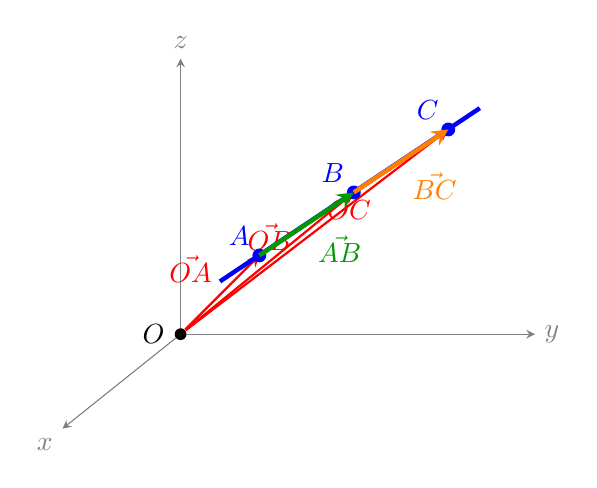
\begin{tikzpicture}[scale=1.0, >=stealth]
    \draw[->, gray] (0,0) -- (-1.5,-1.2) node[below left] {$x$};
    \draw[->, gray] (0,0) -- (4.5,0) node[right] {$y$};
    \draw[->, gray] (0,0) -- (0,3.5) node[above] {$z$};
    \node[circle, fill=black, inner sep=1.5pt, label=left:$O$] (O) at (0,0) {};

    \coordinate (A) at (1,1);
    \coordinate (B) at (2.2,1.8);
    \coordinate (C) at (3.4,2.6);

    \draw[thick, red, ->] (O) -- (A) node[midway, above left] {$\vec{OA}$};
    \draw[thick, red, ->] (O) -- (B) node[midway, above] {$\vec{OB}$};
    \draw[thick, red, ->] (O) -- (C) node[midway, above right] {$\vec{OC}$};

    \draw[ultra thick, blue] (0.5,0.67) -- (3.8,2.87);
    \fill[blue] (A) circle (2.5pt) node[above left] {$A$};
    \fill[blue] (B) circle (2.5pt) node[above left] {$B$};
    \fill[blue] (C) circle (2.5pt) node[above left] {$C$};

    \draw[ultra thick, green!60!black, ->] (A) -- (B) node[midway, below right] {$\vec{AB}$};
    \draw[ultra thick, orange, ->] (B) -- (C) node[midway, below right] {$\vec{BC}$};
\end{tikzpicture}
\end{center}

\vspace{1em}
\noindent\rule{\textwidth}{0.4pt}
\vspace{1em}

% ==================== QUESTION 3 ====================
\subsection*{প্রশ্ন ৩ / Question 3}
\textbf{প্রশ্ন:} xy-তলের উপর অবস্থিত এমন একটি একক ভেক্টর নির্ণয় করো যা $\vec{a} = 2\hat{i} + \hat{j} - 3\hat{k}$ ভেক্টরের উপর লম্ব। [Find a unit vector lying in the xy-plane that is perpendicular to the vector $\vec{a} = 2\hat{i} + \hat{j} - 3\hat{k}$.] [৬]

\vspace{0.8em}
\textbf{সমাধান / Solution:}

ধরি, xy-তলে অবস্থিত যেকোনো ভেক্টর $\vec{b} = x\hat{i} + y\hat{j}$ (যেহেতু এটি xy-তলে অবস্থিত, তাই z-উপাংশ শূন্য)।

যেহেতু $\vec{b}$ ভেক্টরটি $\vec{a}$ এর উপর লম্ব, তাই এদের ডট গুণফল শূন্য হবে:

$$\vec{a} \cdot \vec{b} = 0$$

$$\Rightarrow (2\hat{i} + \hat{j} - 3\hat{k}) \cdot (x\hat{i} + y\hat{j}) = 0$$

$$\Rightarrow 2x + y = 0 \implies y = -2x$$

অতএব, ভেক্টরটি দাঁড়ায়:

$$\vec{b} = x\hat{i} - 2x\hat{j}$$

এখন এই ভেক্টরের অভিমুখে একক ভেক্টর $\hat{b}$ নির্ণয় করি:

$$\hat{b} = \pm \frac{\vec{b}}{|\vec{b}|} = \pm \frac{x\hat{i} - 2x\hat{j}}{\sqrt{x^2 + (-2x)^2}}$$

$$\hat{b} = \pm \frac{x(\hat{i} - 2\hat{j})}{\sqrt{5x^2}} = \pm \frac{1}{\sqrt{5}}(\hat{i} - 2\hat{j})$$

\textbf{উত্তর:} $\pm \frac{1}{\sqrt{5}}(\hat{i} - 2\hat{j})$

\vspace{1em}
\begin{center}
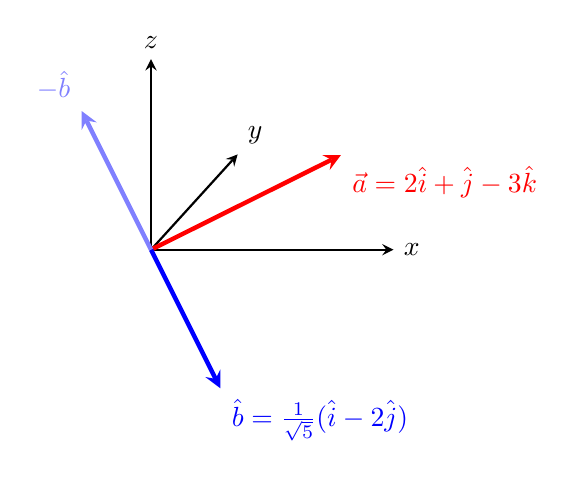
\begin{tikzpicture}[scale=1.1, >=stealth]
    \draw[->, thick] (0,0) -- (2.8,0) node[right] {$x$};
    \draw[->, thick] (0,0) -- (1,1.1) node[above right] {$y$};
    \draw[->, thick] (0,0) -- (0,2.2) node[above] {$z$};

    \draw[->, ultra thick, red] (0,0) -- (1.5,0.4,-1.8) node[below right] {$\vec{a} = 2\hat{i}+\hat{j}-3\hat{k}$};
    \draw[->, ultra thick, blue] (0,0) -- (0.8,-1.6) node[below right] {$\hat{b} = \frac{1}{\sqrt{5}}(\hat{i}-2\hat{j})$};
    \draw[->, ultra thick, blue!50] (0,0) -- (-0.8,1.6) node[above left] {$-\hat{b}$};
\end{tikzpicture}
\end{center}

\vspace{1em}
\noindent\rule{\textwidth}{0.4pt}
\vspace{1em}

% ==================== QUESTION 4 ====================
\subsection*{প্রশ্ন ৪ / Question 4}
\textbf{প্রশ্ন:} $\vec{d}_1$ সরণ ভেক্টরটি yz-তলে y-অক্ষের সাথে $63^\circ$ কোণে অবস্থিত এবং এর z-উপাংশের মান $4.50\text{ m}$। অপর একটি সরণ ভেক্টর $\vec{d}_2$ xz-সমতলে +x অক্ষ হতে $30^\circ$ কোণে অবস্থিত এবং এর z-উপাংশের মান $1.40\text{ m}$। ভেক্টরদ্বয়ের জন্য নির্ণয় করো:
(ক) $\vec{d}_1 \cdot \vec{d}_2$, (খ) $\vec{d}_1 \times \vec{d}_2$ এবং (গ) এদের মধ্যবর্তী কোণ $\theta$। [A displacement vector $\vec{d}_1$ lies in the yz-plane at an angle of $63^\circ$ with the y-axis, and its z-component is $4.50\text{ m}$. Another displacement vector $\vec{d}_2$ lies in the xz-plane at an angle of $30^\circ$ from the +x-axis, and its z-component is $1.40\text{ m}$. Determine for these two vectors: (a) $\vec{d}_1 \cdot \vec{d}_2$, (b) $\vec{d}_1 \times \vec{d}_2$, and (c) the angle $\theta$ between them.] [৬]

\vspace{0.8em}
\textbf{সমাধান / Solution:}

$\vec{d}_1$ ভেক্টরটি yz-তলে অবস্থিত। ধরি, $\vec{d}_1 = y_1\hat{j} + z_1\hat{k}$।

এখানে $z_1 = 4.50\text{ m}$ এবং y-অক্ষের সাথে উৎপন্ন কোণ $63^\circ$:

$$\tan 63^\circ = \frac{z_1}{y_1} = \frac{4.50}{y_1} \implies y_1 = \frac{4.50}{\tan 63^\circ} \approx 2.30\text{ m}$$

অতএব, $\vec{d}_1 = 2.30\hat{j} + 4.50\hat{k}$।

$\vec{d}_2$ ভেক্টরটি xz-তলে অবস্থিত। ধরি, $\vec{d}_2 = x_2\hat{i} + z_2\hat{k}$।

এখানে $z_2 = 1.40\text{ m}$ এবং x-অক্ষের সাথে উৎপন্ন কোণ $30^\circ$:

$$\tan 30^\circ = \frac{z_2}{x_2} = \frac{1.40}{x_2} \implies x_2 = \frac{1.40}{\tan 30^\circ} \approx 2.42\text{ m}$$

অতএব, $\vec{d}_2 = 2.42\hat{i} + 1.40\hat{k}$।

\textbf{(ক) ডট গুণফল ($\vec{d}_1 \cdot \vec{d}_2$):}

$$\vec{d}_1 \cdot \vec{d}_2 = (0\hat{i} + 2.30\hat{j} + 4.50\hat{k}) \cdot (2.42\hat{i} + 0\hat{j} + 1.40\hat{k})$$

$$\vec{d}_1 \cdot \vec{d}_2 = (0 \times 2.42) + (2.30 \times 0) + (4.50 \times 1.40) = 6.30\text{ m}^2$$

\textbf{(খ) ক্রস গুণফল ($\vec{d}_1 \times \vec{d}_2$):}

$$\vec{d}_1 \times \vec{d}_2 = \begin{vmatrix} \hat{i} & \hat{j} & \hat{k} \\ 0 & 2.30 & 4.50 \\ 2.42 & 0 & 1.40 \end{vmatrix}$$

$$= \hat{i}(2.30 \times 1.40 - 0) - \hat{j}(0 - 4.50 \times 2.42) + \hat{k}(0 - 2.30 \times 2.42)$$

$$= 3.22\hat{i} + 10.89\hat{j} - 5.56\hat{k}\text{ m}^2$$

\textbf{(গ) মধ্যবর্তী কোণ ($\theta$):}

$$|\vec{d}_1| = \sqrt{2.30^2 + 4.50^2} \approx 5.05\text{ m}$$

$$|\vec{d}_2| = \sqrt{2.42^2 + 1.40^2} \approx 2.80\text{ m}$$

$$\cos\theta = \frac{\vec{d}_1 \cdot \vec{d}_2}{|\vec{d}_1||\vec{d}_2|} = \frac{6.30}{5.05 \times 2.80} \approx 0.4455$$

$$\theta = \cos^{-1}(0.4455) \approx 63.55^\circ$$

\vspace{1em}
\begin{center}
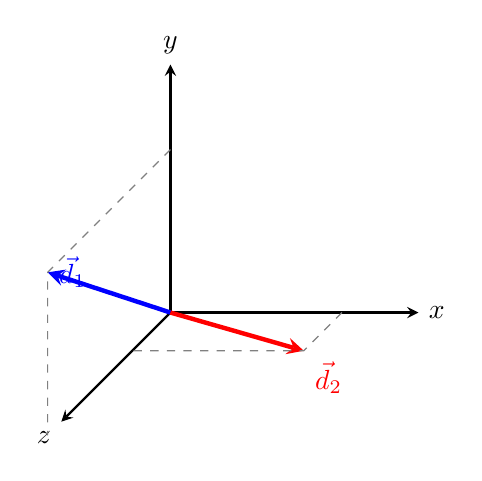
\begin{tikzpicture}[scale=0.9, >=stealth]
    \draw[->, thick] (0,0,0) -- (3.5,0,0) node[right] {$x$};
    \draw[->, thick] (0,0,0) -- (0,3.5,0) node[above] {$y$};
    \draw[->, thick] (0,0,0) -- (0,0,4) node[below left] {$z$};

    \draw[->, ultra thick, blue] (0,0,0) -- (0, 2.3, 4.5) node[right] {$\vec{d}_1$};
    \draw[dashed, gray] (0,2.3,0) -- (0,2.3,4.5) -- (0,0,4.5);

    \draw[->, ultra thick, red] (0,0,0) -- (2.42, 0, 1.4) node[below right] {$\vec{d}_2$};
    \draw[dashed, gray] (2.42,0,0) -- (2.42,0,1.4) -- (0,0,1.4);
\end{tikzpicture}
\end{center}

\vspace{1em}
\noindent\rule{\textwidth}{0.4pt}
\vspace{1em}

% ==================== QUESTION 5 ====================
\subsection*{প্রশ্ন ৫ / Question 5}
\textbf{প্রশ্ন:} যদি তিনটি ভেক্টর যথাক্রমে $\vec{\alpha} = \hat{i} + \hat{j} - 2\hat{k}$, $\vec{\beta} = -\hat{i} + 2\hat{j} + 3\hat{k}$ এবং $\vec{\gamma} = 5\hat{i} + 8\hat{k}$ হয়, তবে স্কেলার রাশি $c$ ও $d$ এর মান নির্ণয় করো যেন, $\vec{\gamma} - c\vec{\alpha} - d\vec{\beta}$ ভেক্টরটি $\vec{\alpha}$ ও $\vec{\beta}$ উভয়ের উপরই লম্ব হয়। [If three vectors are $\vec{\alpha} = \hat{i} + \hat{j} - 2\hat{k}$, $\vec{\beta} = -\hat{i} + 2\hat{j} + 3\hat{k}$, and $\vec{\gamma} = 5\hat{i} + 8\hat{k}$, find the scalar values $c$ and $d$ such that the vector $\vec{\gamma} - c\vec{\alpha} - d\vec{\beta}$ is perpendicular to both $\vec{\alpha}$ and $\vec{\beta}$.] [৬]

\vspace{0.8em}
\textbf{সমাধান / Solution:}

ধরি, নতুন ভেক্টর $\vec{A} = \vec{\gamma} - c\vec{\alpha} - d\vec{\beta}$।

$$\vec{A} = (5\hat{i} + 8\hat{k}) - c(\hat{i} + \hat{j} - 2\hat{k}) - d(-\hat{i} + 2\hat{j} + 3\hat{k})$$

$$\vec{A} = (5 - c + d)\hat{i} - (c + 2d)\hat{j} + (8 + 2c - 3d)\hat{k}$$

যেহেতু $\vec{A}$ ভেক্টরটি $\vec{\alpha}$ এর উপর লম্ব:

$$\vec{A} \cdot \vec{\alpha} = 0 \implies 1(5 - c + d) + 1(-c - 2d) - 2(8 + 2c - 3d) = 0$$

$$\Rightarrow 5 - c + d - c - 2d - 16 - 4c + 6d = 0$$

$$\Rightarrow -6c + 5d = 11 \quad \text{--- (i)}$$

আবার, যেহেতু $\vec{A}$ ভেক্টরটি $\vec{\beta}$ এর উপর লম্ব:

$$\vec{A} \cdot \vec{\beta} = 0 \implies -1(5 - c + d) + 2(-c - 2d) + 3(8 + 2c - 3d) = 0$$

$$\Rightarrow -5 + c - d - 2c - 4d + 24 + 6c - 9d = 0$$

$$\Rightarrow 5c - 14d = -19 \quad \text{--- (ii)}$$

সমীকরণ (i) থেকে পাই, $d = \frac{6c + 11}{5}$। এটি সমীকরণ (ii)-এ বসিয়ে পাই:

$$5c - 14\left(\frac{6c + 11}{5}\right) = -19$$

$$\Rightarrow 25c - 84c - 154 = -95$$

$$\Rightarrow -59c = 59 \implies c = -1$$

$c$ এর মান সমীকরণে বসিয়ে পাই:

$$d = \frac{6(-1) + 11}{5} = 1$$

\textbf{উত্তর:} $c = -1$ এবং $d = 1$

\vspace{1em}
\begin{center}
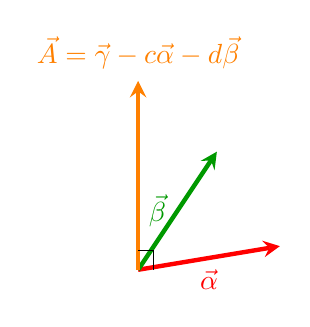
\begin{tikzpicture}[scale=1.0, >=stealth]
    \draw[->, ultra thick, red] (1,0.4) -- (2.8,0.7) node[midway, below] {$\vec{\alpha}$};
    \draw[->, ultra thick, green!60!black] (1,0.4) -- (2,1.9) node[midway, left] {$\vec{\beta}$};
    \draw[->, ultra thick, orange] (1,0.4) -- (1,2.8) node[above] {$\vec{A} = \vec{\gamma} - c\vec{\alpha} - d\vec{\beta}$};
    \draw (1,0.65) -- (1.2,0.65) -- (1.2,0.4);
\end{tikzpicture}
\end{center}

\vspace{1em}
\noindent\rule{\textwidth}{0.4pt}
\vspace{1em}

% ==================== QUESTION 6 ====================
\subsection*{প্রশ্ন ৬ / Question 6}
\textbf{প্রশ্ন:} একটি গতিশীল কণার যেকোনো মুহূর্তের অবস্থান ভেক্টর $\vec{r} = \hat{i}\cos\omega t + \hat{j}\sin\omega t$ দ্বারা নির্দেশ করা যায়, যেখানে $\omega$ একটি ধ্রুবক। কণাটির তাৎক্ষণিক বেগ ও ত্বরণ নির্ণয় করো এবং দেখাও যে, কণাটির অবস্থান ও বেগ ভেক্টরের ক্রস গুণফল $(\vec{r} \times \vec{v})$ একটি ধ্রুবক ভেক্টর। [The position vector of a moving particle at any instant is given by $\vec{r} = \hat{i}\cos\omega t + \hat{j}\sin\omega t$, where $\omega$ is a constant. Find the instantaneous velocity and acceleration of the particle, and show that the cross product of its position and velocity vectors $(\vec{r} \times \vec{v})$ is a constant vector.] [৮]

\vspace{0.8em}
\textbf{সমাধান / Solution:}

১. \textbf{তাৎক্ষণিক বেগ নির্ণয়:}

$$\vec{v} = \frac{d\vec{r}}{dt} = \frac{d}{dt}(\hat{i}\cos\omega t + \hat{j}\sin\omega t) = -\omega\sin\omega t\hat{i} + \omega\cos\omega t\hat{j}$$

২. \textbf{তাৎক্ষণিক ত্বরণ নির্ণয়:}

$$\vec{a} = \frac{d\vec{v}}{dt} = \frac{d}{dt}(-\omega\sin\omega t\hat{i} + \omega\cos\omega t\hat{j}) = -\omega^2\cos\omega t\hat{i} - \omega^2\sin\omega t\hat{j} = -\omega^2\vec{r}$$

৩. \textbf{ক্রস গুণফল $(\vec{r} \times \vec{v})$ নির্ণয়:}

$$\vec{r} \times \vec{v} = \begin{vmatrix} \hat{i} & \hat{j} & \hat{k} \\ \cos\omega t & \sin\omega t & 0 \\ -\omega\sin\omega t & \omega\cos\omega t & 0 \end{vmatrix}$$

$$= \hat{i}(0) - \hat{j}(0) + \hat{k}\left[\cos\omega t(\omega\cos\omega t) - \sin\omega t(-\omega\sin\omega t)\right]$$

$$= \hat{k}\left(\omega\cos^2\omega t + \omega\sin^2\omega t\right) = \omega\hat{k}(\cos^2\omega t + \sin^2\omega t) = \omega\hat{k}$$

যেহেতু $\omega$ এবং একক ভেক্টর $\hat{k}$ উভয়ই সময়-স্বাধীন ধ্রুবক, তাই $\vec{r} \times \vec{v} = \omega\hat{k}$ একটি ধ্রুবক ভেক্টর। *(দেখানো হলো)*

\vspace{1em}
\begin{center}
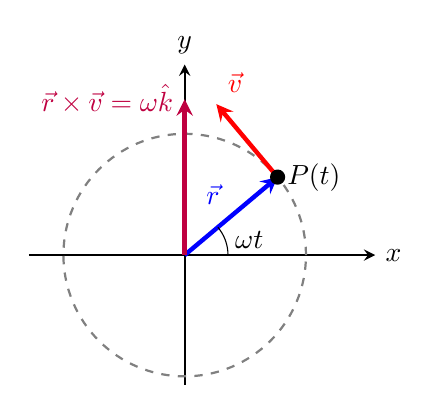
\begin{tikzpicture}[scale=1.1, >=stealth]
    \draw[->, thick] (-1.8,0) -- (2.2,0) node[right] {$x$};
    \draw[->, thick] (0,-1.5) -- (0,2.2) node[above] {$y$};
    \draw[dashed, thick, gray] (0,0) circle (1.4);

    \coordinate (P) at (40:1.4);
    \draw[->, ultra thick, blue] (0,0) -- (P) node[midway, above left] {$\vec{r}$};
    \draw[->, ultra thick, red] (P) -- ($(P)+(130:1.1)$) node[above right] {$\vec{v}$};
    \fill (P) circle (2.5pt) node[right] {$P(t)$};

    \draw[->, ultra thick, purple] (0,0) -- (0,1.8) node[left] {$\vec{r}\times\vec{v} = \omega\hat{k}$};
    \draw (0.5,0) arc (0:40:0.5) node[midway, right] {$\omega t$};
\end{tikzpicture}
\end{center}

\vspace{1em}
\noindent\rule{\textwidth}{0.4pt}
\vspace{1em}

% ==================== QUESTION 7 ====================
\subsection*{প্রশ্ন ৭ / Question 7}
\textbf{প্রশ্ন:} যদি রৈখিক বেগ $\vec{v} = \vec{\omega} \times \vec{r}$ হয়, তবে ভেক্টর ক্যালকুলাসের কার্ল (Curl) সূত্র ব্যবহার করে প্রমাণ করো যে, কৌণিক বেগ $\vec{\omega} = \frac{1}{2}(\vec{\nabla} \times \vec{v})$। এখানে $\vec{\omega}$ একটি ধ্রুব কৌণিক বেগ ভেক্টর এবং $\vec{r} = x\hat{i} + y\hat{j} + z\hat{k}$ হলো অবস্থান ভেক্টর। [If the linear velocity is $\vec{v} = \vec{\omega} \times \vec{r}$, prove using the curl formula of vector calculus that the angular velocity is $\vec{\omega} = \frac{1}{2}(\vec{\nabla} \times \vec{v})$. Here $\vec{\omega}$ is a constant angular velocity vector and $\vec{r} = x\hat{i} + y\hat{j} + z\hat{k}$ is the position vector.] [৯]

\vspace{0.8em}
\textbf{সমাধান / Solution:}

ধরি, ধ্রুব কৌণিক বেগ ভেক্টর $\vec{\omega} = \omega_x\hat{i} + \omega_y\hat{j} + \omega_z\hat{k}$ এবং অবস্থান ভেক্টর $\vec{r} = x\hat{i} + y\hat{j} + z\hat{k}$।

প্রথমে $\vec{v}$ নির্ণয় করি:

$$\vec{v} = \vec{\omega} \times \vec{r} = \begin{vmatrix} \hat{i} & \hat{j} & \hat{k} \\ \omega_x & \omega_y & \omega_z \\ x & y & z \end{vmatrix}$$

$$\vec{v} = \hat{i}(\omega_y z - \omega_z y) - \hat{j}(\omega_x z - \omega_z x) + \hat{k}(\omega_x y - \omega_y x)$$

এখন, $\vec{v}$ এর কার্ল ($\vec{\nabla} \times \vec{v}$) নির্ণয় করি:

$$\vec{\nabla} \times \vec{v} = \begin{vmatrix} \hat{i} & \hat{j} & \hat{k} \\ \frac{\partial}{\partial x} & \frac{\partial}{\partial y} & \frac{\partial}{\partial z} \\ \omega_y z - \omega_z y & \omega_z x - \omega_x z & \omega_x y - \omega_y x \end{vmatrix}$$

$\hat{i}$-উপাংশ:

$$\frac{\partial}{\partial y}(\omega_x y - \omega_y x) - \frac{\partial}{\partial z}(\omega_z x - \omega_x z) = \omega_x - (-\omega_x) = 2\omega_x$$

$\hat{j}$-উপাংশ:

$$-\left[\frac{\partial}{\partial x}(\omega_x y - \omega_y x) - \frac{\partial}{\partial z}(\omega_y z - \omega_z y)\right] = -(-\omega_y - \omega_y) = 2\omega_y$$

$\hat{k}$-উপাংশ:

$$\frac{\partial}{\partial x}(\omega_z x - \omega_x z) - \frac{\partial}{\partial y}(\omega_y z - \omega_z y) = \omega_z - (-\omega_z) = 2\omega_z$$

অতএব:

$$\vec{\nabla} \times \vec{v} = 2\omega_x\hat{i} + 2\omega_y\hat{j} + 2\omega_z\hat{k} = 2\vec{\omega}$$

$$\Rightarrow \vec{\omega} = \frac{1}{2}(\vec{\nabla} \times \vec{v}) \quad \text{*(প্রমাণিত)*}$$

\vspace{1em}
\begin{center}
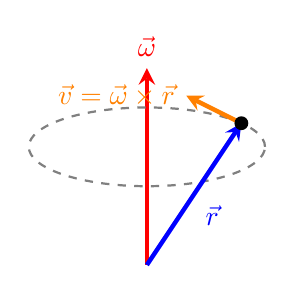
\begin{tikzpicture}[scale=1.0, >=stealth]
    \draw[->, ultra thick, red] (0,0) -- (0,2.5) node[above] {$\vec{\omega}$};
    \draw[dashed, thick, gray] (0,1.5) ellipse (1.5 and 0.5);
    \coordinate (P) at (1.2, 1.8);
    \draw[->, ultra thick, blue] (0,0) -- (P) node[midway, below right] {$\vec{r}$};
    \draw[->, ultra thick, orange] (P) -- ($(P)+(-0.7,0.35)$) node[left] {$\vec{v} = \vec{\omega}\times\vec{r}$};
    \fill (P) circle (2.5pt);
\end{tikzpicture}
\end{center}

\vspace{1em}
\noindent\rule{\textwidth}{0.4pt}
\vspace{1em}

% ==================== QUESTION 8 ====================
\subsection*{প্রশ্ন ৮ / Question 8}
\textbf{প্রশ্ন:} ভেক্টর ক্যালকুলাসের অত্যন্ত গুরুত্বপূর্ণ একটি উপপাদ্য হলো "যেকোনো ভেক্টর ক্ষেত্রের কার্লের ডাইভারজেন্স সর্বদা শূন্য"। গাণিতিকভাবে প্রমাণ করো যে, $\vec{\nabla} \cdot (\vec{\nabla} \times \vec{A}) = 0$। [A crucial theorem of vector calculus states that "the divergence of the curl of any vector field is always zero." Mathematically prove that $\vec{\nabla} \cdot (\vec{\nabla} \times \vec{A}) = 0$.] [১০]

\vspace{0.8em}
\textbf{সমাধান / Solution:}

ধরি, যেকোনো ভেক্টর ক্ষেত্র $\vec{A} = A_x\hat{i} + A_y\hat{j} + A_z\hat{k}$।

প্রথমে $\vec{A}$ এর কার্ল নির্ণয় করি:

$$\vec{\nabla} \times \vec{A} = \hat{i}\left(\frac{\partial A_z}{\partial y} - \frac{\partial A_y}{\partial z}\right) + \hat{j}\left(\frac{\partial A_x}{\partial z} - \frac{\partial A_z}{\partial x}\right) + \hat{k}\left(\frac{\partial A_y}{\partial x} - \frac{\partial A_x}{\partial y}\right)$$

এখন এই কার্লের ডাইভারজেন্স ($\vec{\nabla} \cdot$) নির্ণয় করি:

$$\vec{\nabla} \cdot (\vec{\nabla} \times \vec{A}) = \frac{\partial}{\partial x}\left(\frac{\partial A_z}{\partial y} - \frac{\partial A_y}{\partial z}\right) + \frac{\partial}{\partial y}\left(\frac{\partial A_x}{\partial z} - \frac{\partial A_z}{\partial x}\right) + \frac{\partial}{\partial z}\left(\frac{\partial A_y}{\partial x} - \frac{\partial A_x}{\partial y}\right)$$

$$= \frac{\partial^2 A_z}{\partial x \partial y} - \frac{\partial^2 A_y}{\partial x \partial z} + \frac{\partial^2 A_x}{\partial y \partial z} - \frac{\partial^2 A_z}{\partial y \partial x} + \frac{\partial^2 A_y}{\partial z \partial x} - \frac{\partial^2 A_x}{\partial z \partial y}$$

আংশিক অন্তরীকরণের ক্রম পরিবর্তনশীলতার উপপাদ্যানুসারে ($\frac{\partial^2 f}{\partial x \partial y} = \frac{\partial^2 f}{\partial y \partial x}$):

$$\vec{\nabla} \cdot (\vec{\nabla} \times \vec{A}) = \left(\frac{\partial^2 A_z}{\partial x \partial y} - \frac{\partial^2 A_z}{\partial y \partial x}\right) + \left(\frac{\partial^2 A_y}{\partial z \partial x} - \frac{\partial^2 A_y}{\partial x \partial z}\right) + \left(\frac{\partial^2 A_x}{\partial y \partial z} - \frac{\partial^2 A_x}{\partial z \partial y}\right) = 0$$

অতএব, যেকোনো ভেক্টর ক্ষেত্রের কার্লের ডাইভারজেন্স সর্বদা শূন্য। *(প্রমাণিত)*

\vspace{1em}
\begin{center}
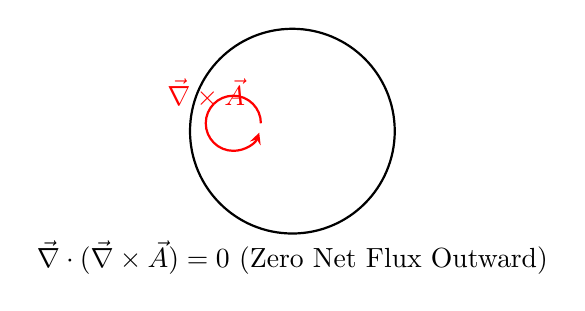
\begin{tikzpicture}[scale=1.0, >=stealth]
    \draw[thick] (0,0) circle (1.3);
    \draw[->, thick, red] (-0.4,0.1) arc (0:340:0.35) node[midway, above] {$\vec{\nabla}\times\vec{A}$};
    \node at (0,-1.6) {$\vec{\nabla} \cdot (\vec{\nabla} \times \vec{A}) = 0$ (Zero Net Flux Outward)};
\end{tikzpicture}
\end{center}

\vspace{1em}
\noindent\rule{\textwidth}{0.4pt}
\vspace{1em}

% ==================== QUESTION 9 ====================
\subsection*{প্রশ্ন ৯ / Question 9}
\textbf{প্রশ্ন:} যদি $\vec{r} = x\hat{i} + y\hat{j} + z\hat{k}$ অবস্থান ভেক্টর এবং $r = |\vec{r}|$ এর মান হয়, তবে ডাইভারজেন্স ও গ্রেডিয়েন্টের সম্পর্ক ব্যবহার করে $\vec{\nabla} \cdot (r^3\vec{r})$ এর মান নির্ণয় করো। [If $\vec{r} = x\hat{i} + y\hat{j} + z\hat{k}$ is the position vector and $r = |\vec{r}|$ is its magnitude, determine the value of $\vec{\nabla} \cdot (r^3\vec{r})$ using the relationship between divergence and gradient.] [১১]

\vspace{0.8em}
\textbf{সমাধান / Solution:}

আমরা জানি ভেক্টর অভেদ:

$$\vec{\nabla} \cdot (\phi \vec{F}) = \phi (\vec{\nabla} \cdot \vec{F}) + \vec{F} \cdot (\vec{\nabla} \phi)$$

এখানে, $\phi = r^3$ এবং $\vec{F} = \vec{r}$।

১. আমরা জানি:

$$\vec{\nabla} \cdot \vec{r} = \frac{\partial x}{\partial x} + \frac{\partial y}{\partial y} + \frac{\partial z}{\partial z} = 1 + 1 + 1 = 3$$

২. $r^3$ এর গ্রেডিয়েন্ট ($\vec{\nabla} r^3$) নির্ণয় করি:

$$\vec{\nabla}(r^3) = 3r^2 \vec{\nabla}(r)$$

যেহেতু $\vec{\nabla}(r) = \frac{\vec{r}}{r}$ (অবস্থান ভেক্টরের মান $r$ এর গ্রেডিয়েন্ট), সেহেতু:

$$\vec{\nabla}(r^3) = 3r^2 \frac{\vec{r}}{r} = 3r\vec{r}$$

এখন মূল সূত্রে মানগুলো বসিয়ে পাই:

$$\vec{\nabla} \cdot (r^3\vec{r}) = r^3 (\vec{\nabla} \cdot \vec{r}) + \vec{r} \cdot (\vec{\nabla} r^3)$$

$$= r^3 (3) + \vec{r} \cdot (3r\vec{r})$$

$$= 3r^3 + 3r (\vec{r} \cdot \vec{r})$$

যেহেতু $\vec{r} \cdot \vec{r} = r^2$:

$$= 3r^3 + 3r(r^2) = 3r^3 + 3r^3 = 6r^3$$

\textbf{উত্তর:} $6r^3$

\vspace{1em}
\begin{center}
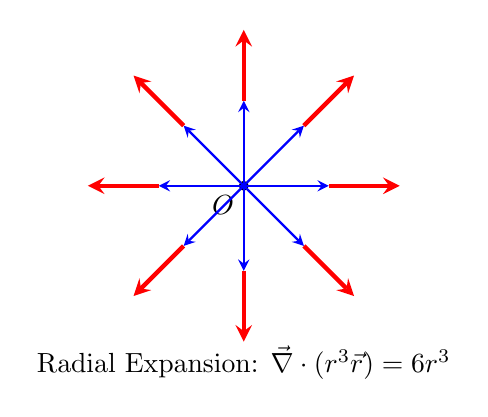
\begin{tikzpicture}[scale=0.9, >=stealth]
    \fill (0,0) circle (2pt) node[below left] {$O$};
    \foreach \angle in {0, 45, 90, 135, 180, 225, 270, 315} {
        \draw[->, thick, blue] (0,0) -- (\angle:1.2);
        \draw[->, ultra thick, red] (\angle:1.2) -- (\angle:2.2);
    }
    \node at (0,-2.5) {Radial Expansion: $\vec{\nabla} \cdot (r^3\vec{r}) = 6r^3$};
\end{tikzpicture}
\end{center}

\vspace{1em}
\noindent\rule{\textwidth}{0.4pt}
\vspace{1em}

% ==================== QUESTION 10 ====================
\subsection*{প্রশ্ন ১০ / Question 10}
\textbf{প্রশ্ন:} ত্রিমাত্রিক ভেক্টর ক্ষেত্র $\vec{E} = \frac{\vec{r}}{r^2}$ এর জন্য কার্ল (Curl) নির্ণয় করে দেখাও যে, ভেক্টর ক্ষেত্রটি অঘূর্ণনশীল (irrotational)। এখানে $\vec{r} = x\hat{i} + y\hat{j} + z\hat{k}$ এবং $r = \sqrt{x^2+y^2+z^2}$। [Find the curl for the three-dimensional vector field $\vec{E} = \frac{\vec{r}}{r^2}$ and show that the vector field is irrotational. Here $\vec{r} = x\hat{i} + y\hat{j} + z\hat{k}$ and $r = \sqrt{x^2+y^2+z^2}$.] [১২]

\vspace{0.8em}
\textbf{সমাধান / Solution:}

প্রথমে ভেক্টর ক্ষেত্রটিকে কার্তেসীয় উপাংশে রূপান্তর করি:

$$\vec{E} = \frac{x\hat{i} + y\hat{j} + z\hat{k}}{x^2 + y^2 + z^2} = E_x\hat{i} + E_y\hat{j} + E_z\hat{k}$$

এখানে:

$$E_x = \frac{x}{x^2+y^2+z^2}, \quad E_y = \frac{y}{x^2+y^2+z^2}, \quad E_z = \frac{z}{x^2+y^2+z^2}$$

অঘূর্ণনশীল প্রমাণ করতে আমাদের দেখাতে হবে যে $\vec{\nabla} \times \vec{E} = \vec{0}$।

$$\vec{\nabla} \times \vec{E} = \begin{vmatrix} \hat{i} & \hat{j} & \hat{k} \\ \frac{\partial}{\partial x} & \frac{\partial}{\partial y} & \frac{\partial}{\partial z} \\ \frac{x}{x^2+y^2+z^2} & \frac{y}{x^2+y^2+z^2} & \frac{z}{x^2+y^2+z^2} \end{vmatrix}$$

$\hat{i}$-উপাংশটি হিসাব করি:

$$\frac{\partial E_z}{\partial y} - \frac{\partial E_y}{\partial z} = \frac{\partial}{\partial y}\left(\frac{z}{x^2+y^2+z^2}\right) - \frac{\partial}{\partial z}\left(\frac{y}{x^2+y^2+z^2}\right)$$

$$= \frac{-2yz}{(x^2+y^2+z^2)^2} - \left(\frac{-2yz}{(x^2+y^2+z^2)^2}\right) = 0$$

একইভাবে প্রতিসাম্যতার (symmetry) কারণে $\hat{j}$ এবং $\hat{k}$ উপাংশদ্বয়ও শূন্য হবে:

$$\text{Curl }\vec{E} = \vec{\nabla} \times \vec{E} = 0\hat{i} + 0\hat{j} + 0\hat{k} = \vec{0}$$

যেহেতু কার্লের মান একটি শূন্য ভেক্টর, তাই $\vec{E} = \frac{\vec{r}}{r^2}$ ভেক্টর ক্ষেত্রটি অঘূর্ণনশীল (irrotational)। *(দেখানো হলো)*

\vspace{1em}
\begin{center}
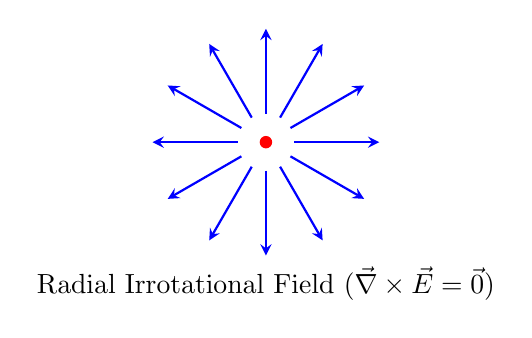
\begin{tikzpicture}[scale=0.9, >=stealth]
    \fill[red] (0,0) circle (2.5pt);
    \foreach \angle in {0, 30, 60, 90, 120, 150, 180, 210, 240, 270, 300, 330} {
        \draw[->, thick, blue] (\angle:0.4) -- (\angle:1.6);
    }
    \node at (0,-2.0) {Radial Irrotational Field ($\vec{\nabla} \times \vec{E} = \vec{0}$)};
\end{tikzpicture}
\end{center}

\end{document}